\section{Controlerkomponente VCM-Wrapper}
\subsection{Zusammenfassung}
Der VCM-Wrapper spiegelt der Eclipse-Plattform ein vollfunktionsf�higes Team-
Plugin vor, �ber das alle Repositoryoperationen durchgef�hrt werden. Intern
gibt die Komponente die Aktionen jedoch an andere Team-Plugins weiter. Vor und
nach jeder dieser Aktion wird die Kommunikations-Komponente konsultiert, um 
den Server bzw. andere Clients �ber Ver�nderungen am Repository zu 
informieren. Die VCM-Wrapper-Komponente kennt sowohl die Datei-Ebene und deren
Repositories als auch die Abstraktion auf Produktlinien/Komponenten/Varianten.
F�r beide Ebenen lassen sich atomare (z.B. checkin) und komplexe VCM-
Aktionen () ausf�hren. Die n�tigen Informationen �ber 
Repository-Positionen und Struktur bezieht der VCM-Wrapper �ber die Server-
Kommunikations-Komponente sowie das Architekturmodel.

%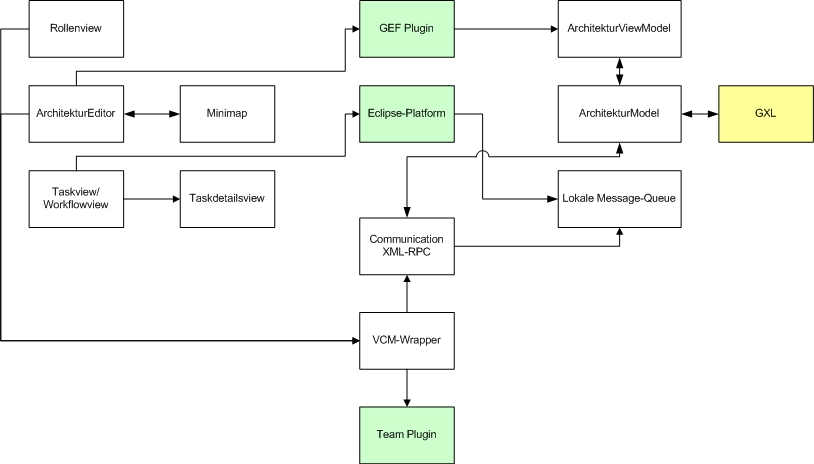
\includegraphics[width=15cm]{client.jpg}

\subsection{Manueller Import der Einstellungen}
Der Client st�� die Delegater-Schicht an. Als positives Ergebnis sind
alle Konfigurationsdaten in Eclipse gespeichert. 
\par 
Durch diese Konfigurationsdaten kann Eclipse entscheiden welche
Repositories, zugeh�rige Rollen und Zugriffsrechte benutzt werden
m�ssen.
Dadurch k�nnen in Eclipse durch die erhaltenen Rollen und
Repository-Daten die vordefinierten Felder zum Zugriff auf
VCM-Repositories entsprechend gesetzt werden. Hierdurch wird eine
optimale Anbindung an bereits existierende Eclipse-Strukturen
geschaffen. 

\subsection{Automatischer Import der Einstellungen}
Falls der Benutzer das erste Mal Eclipse startet, d.h. noch keine
Konfigurationsdaten zu Rollen und Repositories vorliegen, wird die
delegater-Schicht automatisch angesto�en, und die Konfigurationsdaten
vom Server geladen und in Eclipsae gepeichert, wie im manuellen
Import n�her beschrieben.

\subsection{Ablaufschritte beim Zugriff auf das Repository}

Die Ablaufschritte:\par

\begin{itemize}
    \item Lade Konfigurationsdaten vom Server (fetch)
    \item Extrahiere Rollenzuteilung, Repository-Daten
    \item Lokale Pr�fung auf vorhandenes Produkt, d.h. Produktdaten, Benutzerdaten (check)
    \item Pr�fungsergebnisse f�hren bei nicht vorhandenem Produkt zu
    �ffnendem Dialog und anschlie�ender Lade-Aktion (checkout) aus dem
    Repository
\end{itemize}\par

\subsection{M�gliche Wrapper-Aktionen}

Alle m�glichen Wrapper-Aktionen lassen sich in zwei verschiedene
Gruppen einteilen. Aktionen die keine Berechtigung erfordern, d.h. f�r
alle Benutzer m�glich sind und Aktionen die eine Berechtigung
erfordern, d.h. nur f�r bestimmte m�glich sind.\par

Die sichtbaren Aktionen:\par

\bf Alle Benutzer:
\begin{itemize}
  \item check out: immer m�glich, ggf. nur Leserechte.
  \item update: Vorbedingung: check out
\end{itemize}

\bf Nur bestimmte Benutzer:

\begin{itemize}
  \item commit: Vorbedingung: check out
  \item import: in der ersten Iteration nicht m�glich!
  \item delete: -
  \item add: -
\end{itemize}

Falls eine Aktion der zweiten Gruppe nicht erfolgreich ausgef�hrt
werden kann, entweder weil der Client feststellt dass der Benutzer
nicht die passende Rolle besitzt, d.h. eine unerlaubte Aktion
angesto�en wurde oder weil der Repository-Server beim durchf�hren der
Aktion eine Fehlermeldung zur�ck gibt wird auf dem Server ein
passender Workflow der zu dem speziellen Feedback passt, angestossen.


\subsection{Skriptausf�hrung}
Allen m�glichen Wrapper-Aktionen kann zus�tzlich eine bestimmte
Matainfo-Datei �bergeben werden, das eine georndete Liste von Skripten
enth�lt, die vor und nach einem ``commit'' ausgef�hrt werden. Diese
m�glichen Metainfo-Dateien werden an anderer Stelle festgelegt.

\subsection{Konsistenzcheck bei der Produktzusammenstellung}
Als Konsistenzcheck wird die Anfrage an die Datenbasis genannt, die
als Eingabeparameter die Revision oder den Autor einer bestimmten
Datei xy erh�lt und zur�ckgibt ob die Datei vorhanden (match=syncron)
ist (oder nicht) und ob die Revision �bereinstimmt. Ggf. wird ein
passender Workflow angesto�en.\par
Zur �berpr�fung des gesamten Produktes werden oben genannte Schritte
angewandt, wobei die Eingabemenge aus Dateinamen und deren Revisionen
besteht.

\subsection{der initial Metadaten-Abgleich}
Vorbedingung:...

\subsection{Einschr�nkungen bei der Implementierung}
